\documentclass[11pt]{article}
\usepackage[paper=letterpaper, left=1.25in, right=1.25in, top=1.25in, bottom=1.25in]
           {geometry}
\usepackage[parfill]{parskip}
\usepackage{amsmath}
\usepackage{graphicx}
\usepackage{fancyvrb}
\usepackage{upquote}
\usepackage{xfrac}

\newcommand{\problem}[1]{\textbf{Problem #1 ---} }
\newcommand{\answer}{\textit{Answer: } }

\begin{document}
\thispagestyle{empty}

\begin{center}
CS310 -- Assignment 228 -- Karl Ramberg
\end{center}

Quicksort is only as good as its partition function so analyzing different
approaches for partitioning is super important.

Let's look at the two provided partition functions, \texttt{partition\_j()}
and \texttt{partition\_w()}. Both \texttt{partition\_j()} and
\texttt{partition\_w()} have and input size of $n$ where $n$ is the difference
between \texttt{hi} and \texttt{lo}. When dealing with a \texttt{vector} our
input size usually corresponds with the \texttt{vector} size, but both
partition algortithms will only look at values between \texttt{a.at(lo)} and
\texttt{a.at(hi)}.

\begin{center}
\line(1,0){100}
\end{center}

Let's look at \texttt{partition\_j()} in detail first.

\texttt{partition\_j()} has one main \texttt{if} statement, but this only takes care of
a few special cases, namely a singleton \texttt{vector} and a \texttt{vector}
of size $0$. We won't count these special cases in our analysis. This means
we should only care what is inside the \texttt{if} block.

The \texttt{if} comparisons themeselves are $3$ operations. Inside the block
there are $2$ more before we reach a \texttt{for} loop. The body of the loop
will run $n-1$ times since we start \texttt{index} at \texttt{lo + 1} and the
header will run an additional time in order to exit.

Inside the \texttt{for} loop there is a single \texttt{if} statement. The loop
body will always do that $1$ comparison and $3$ additional if the comparison
was true -- $1$ arthimatic operation and $2$ for a swap.

This means the formal formulations of the number of basic operations as a
function of input size is $T(n) = 6n + 7$ for worst case (swap every time) and
$T(n) = 3n + 7$ for best case (no swaps needed).

These are both of the same efficiency class so we can conclude
\[
T(n) \in \Theta(n)
\]

I ran \texttt{partition\_j()} many times with many different input sizes  and
scaled standard functions in order to illustrate this. Here are the results
graphed with gnuplot...

\begin{center}
  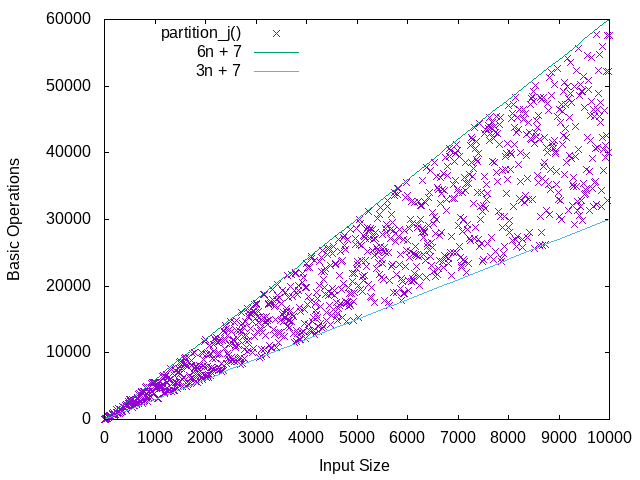
\includegraphics[width=0.525\textwidth]{p1_1.png}
\end{center}

\begin{center}
\line(1,0){100}
\end{center}

Now let's look at \texttt{partition\_w()} in detail.

\texttt{partition\_w()} has one main \texttt{if} structure just like
\texttt{partition\_j()}. We can ignore the first \texttt{if} and
\texttt{else if} because they deal with special cases of a \texttt{hi} and
\texttt{lo} being invalid or only being $1$ or $2$ apart. However we should
count the $5$ comparisons needed to find the normal case.

Inside the normal case there are $4$ various operations before a
\texttt{while} loop. The \texttt{while} loop runs based on two markers,
\texttt{left} and \texttt{right} the approach eachother from opposite sides of
the \texttt{vector}. The elements at \texttt{left} and \texttt{right} will
swap places if they are on the wrong side of the pivot.

For the worst case that the \texttt{vector} is reversed, the outer
\texttt{while} will run $n$ times and each inner \texttt{while} loop will only
run once each time since the next value will alawys be on the wrong side.

For the best case, the outer loop will only run once since the inner loops
will cross there markers on the first pass.

This means that each set of loops, outer and inner, will run more or less
based on the input arrangment. However this means that if one runs fewer times
the other will run more. This means the algorithm is not more complex simply
because there are nested loops.

For the worst case (outer loop run $n$ times) the number of basic operations
as a function of input looks like so: $T(n) = 6n + 11$. For the best case
(inner loops run $n$ times combined) the number of basic operations as a
function of input size looks like so: $T(n) = 2n + 20$.

These are both of the same efficiency class so we can conclude
\[
T(n) \in \Theta(n)
\]

I ran \texttt{partition\_w()} many times with many different input sizes and
scaled standard functions in order to illustrate this. Here are the results
graphed with gnuplot...

\begin{center}
  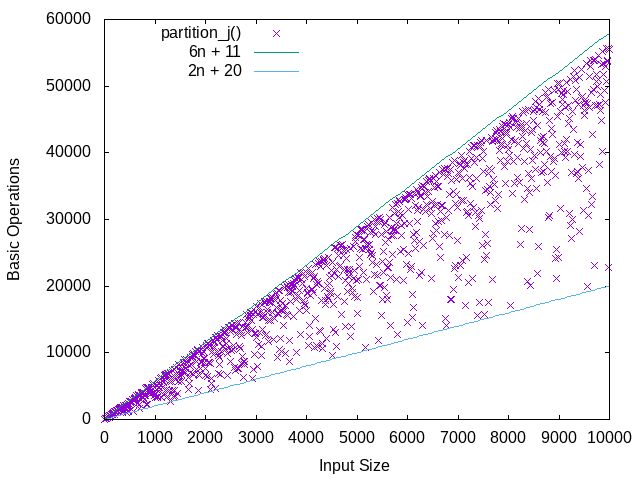
\includegraphics[width=0.525\textwidth]{p1_2.png}
\end{center}

\begin{center}
\line(1,0){100}
\end{center}

We can modify both of these paritioning functions to group all the duplicate
pivots together. I modified \texttt{partitiion\_j()} to show this. You can see
the modified version at \texttt{partition\_j\_modified.cpp}. I did this by
moving any dupliates of the pivot next to the original and swap all pivots to
there position when everything else is in order. This added a few operations
and a \texttt{for} loop for swapping the pivots at the end. This loop will run
a maximum of $n$ times when all elements are the same as the pivot. This means
out complexity won't change. Here is the efficiency of the modifcations 
graphed with gnuplot...

\begin{center}
  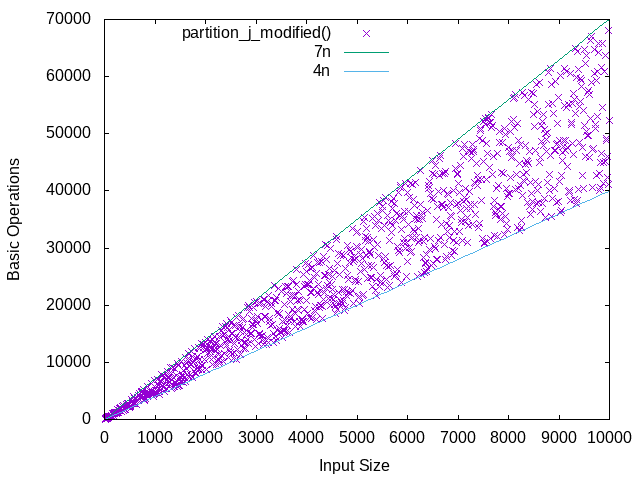
\includegraphics[width=0.525\textwidth]{p2.png}
\end{center}

\end{document}




%%  LocalWords:  cn Yada yada indx cerr cpp dat